\documentclass[hyperref=colorlinks]{beamer}
\mode<presentation>
\usetheme{iclpt}
\setbeamertemplate{navigation symbols}{}
\setbeamertemplate{headline}{
  \begin{beamercolorbox}[leftskip=.2cm,rightskip=.2cm,topskip=.2cm,ht=1.1cm,dp=0.1cm,wd=\textwidth]{institute in head/foot}
    
\includegraphics[height=1cm]{icl.pdf}
    \hfill
%    \includegraphics[height=1cm]{../Pics/ATLAS-Logo-Square-Blue-RGB.png}
%    
\includegraphics[height=1cm]{../Pics/CMS-Color.pdf}
    
\includegraphics[height=1cm]{TalkPics/t2k_logo_large.png}

%??put t2k logo here
  \end{beamercolorbox}
}
\setbeamertemplate{footline}{
  \begin{beamercolorbox}[ht=.35cm,dp=0.2cm,wd=\textwidth,leftskip=.3cm]{author in head/foot}%
    \begin{minipage}[c]{5cm}%
      \usebeamerfont{author in head/foot}
      \insertshortauthor 
      \insertshorttitle
    \end{minipage}\hfill%
    \hfill
    \insertframenumber{} / \ref{lastframe}
    %\hfill
    \begin{minipage}{6cm}
      \hfill
      %\insertshorttitle
    \end{minipage}
  \end{beamercolorbox}%
}

\definecolor{beamer@icdarkblue}{RGB}{0,51,102}
\definecolor{beamer@icmiddleblue}{RGB}{0,82,150} 
\definecolor{beamer@iclightblue}{RGB}{200,212,232}
\definecolor{beamer@icmiddlered}{RGB}{204,51,0}
\definecolor{beamer@iclightred}{RGB}{232,212,32}

\usepackage{tikz}
\usetikzlibrary{arrows,shapes,backgrounds}
\usepackage{color}
\usepackage{tabularx,colortbl}
\usepackage{graphicx}
\usepackage{pdfpages}
\usepackage{feynmp}
\usepackage{rotating}
\usepackage{moresize}
\usepackage{slashed}
\usepackage{xcolor,colortbl}
\DeclareGraphicsRule{*}{mps}{*}{}
\hypersetup{colorlinks=false}

\title[Transverse Variables for HPTPC]{\vspace{-0.2cm} Transverse Variables for HPTPC}
\author[P. Dunne]{Patrick Dunne - Imperial College London}
\titlegraphic{
  \vspace{-0.4cm}
}
\date{}
\begin{document}
\tikzstyle{every picture}+=[remember picture]
\tikzstyle{na} = [baseline=-.5ex]
\begin{fmffile}{t2ktemplatefeyndiags}


  %TITLE PAGE
  %20 mins + 5 questions
  \section{Title}
  \begin{frame}
    \titlepage
  \end{frame}

  \begin{frame}
    \frametitle{Overview}
    \begin{block}{}
        \scriptsize
        \begin{itemize}
        \item Update on previous presentation on Single Transverse Variables (STV)
        \item[-] Now have 2D distributions and weighting for target mass in HPTPC ND280 comparisons
        \item Reminder of STV
        \item Distributions of STV for ND280 and HPTPC-like selections focussing on CC0$\pi$1p
      \end{itemize}
    \end{block}
  \end{frame}

  \begin{frame}
    \frametitle{Single Transverse Variables}
    \begin{itemize}
    \item Use hadronic information to estimate nuclear effects
    \item For simple CCQE without nuclear effects $\delta p_{T}=0$, $\delta \alpha_{T}=\pi$, $\delta \phi_{T}=0$ 
    \end{itemize}
    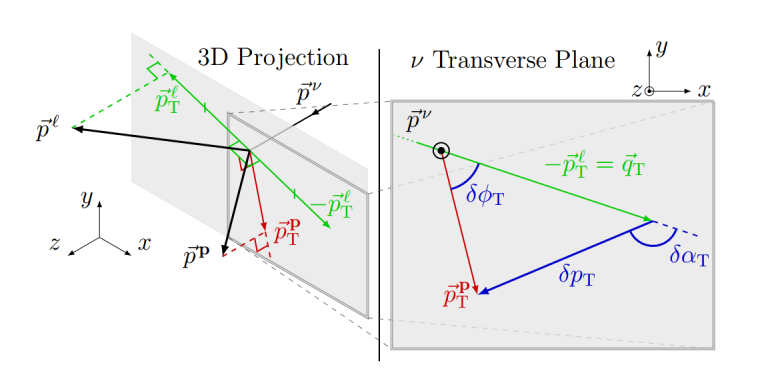
\includegraphics[width=\textwidth]{TalkPics/STVforHPTPC_101016/stvdiagram.png}
  \end{frame}

  \begin{frame}
    \frametitle{HPTPC Study}
    \begin{itemize}
    \item HPTPC-like and ND280-like momentum thresholds (below) and efficiencies (see Mark's talk 10th October) were applied to ND280 MC truth
    \item[-] Same as shown previously
    \item HPTPC sample then weighted by 635/2202 to account for target mass
    \item Then calculated transverse variables
    \item[-] Only make sense in samples with a proton or a pion
    \end{itemize}
    \begin{tabular}{l|cc}
      \hline
      Particle & ND280 Threshold/MeV & HPTPC Threshold/MeV \\
      \hline
      $\mu$ & 100 & 15 \\
      $\pi$ & 120 & 16 \\
      $p$ & 450 & 60 \\
      $e$ & 100 & 1 \\
      \hline
    \end{tabular}
  \end{frame}

  \begin{frame}
    \frametitle{HPTPC Study}
    \begin{itemize}
    \item Truth information is used to determine which events truly belong in the sample (``correct''), and which are ``fakes''
    \item[-] Distributions of transverse variables are shown for both
    \item Saw last time that distributions of transverse variables were similar between ND280 and HPTPC, but much lower fake rate
    \item Will investigate 2D distributions with each other and other kinematic variables
    \end{itemize}
  \end{frame}

  \begin{frame}
    \frametitle{1D distributions for CC0$\pi$1p}
    \centering
    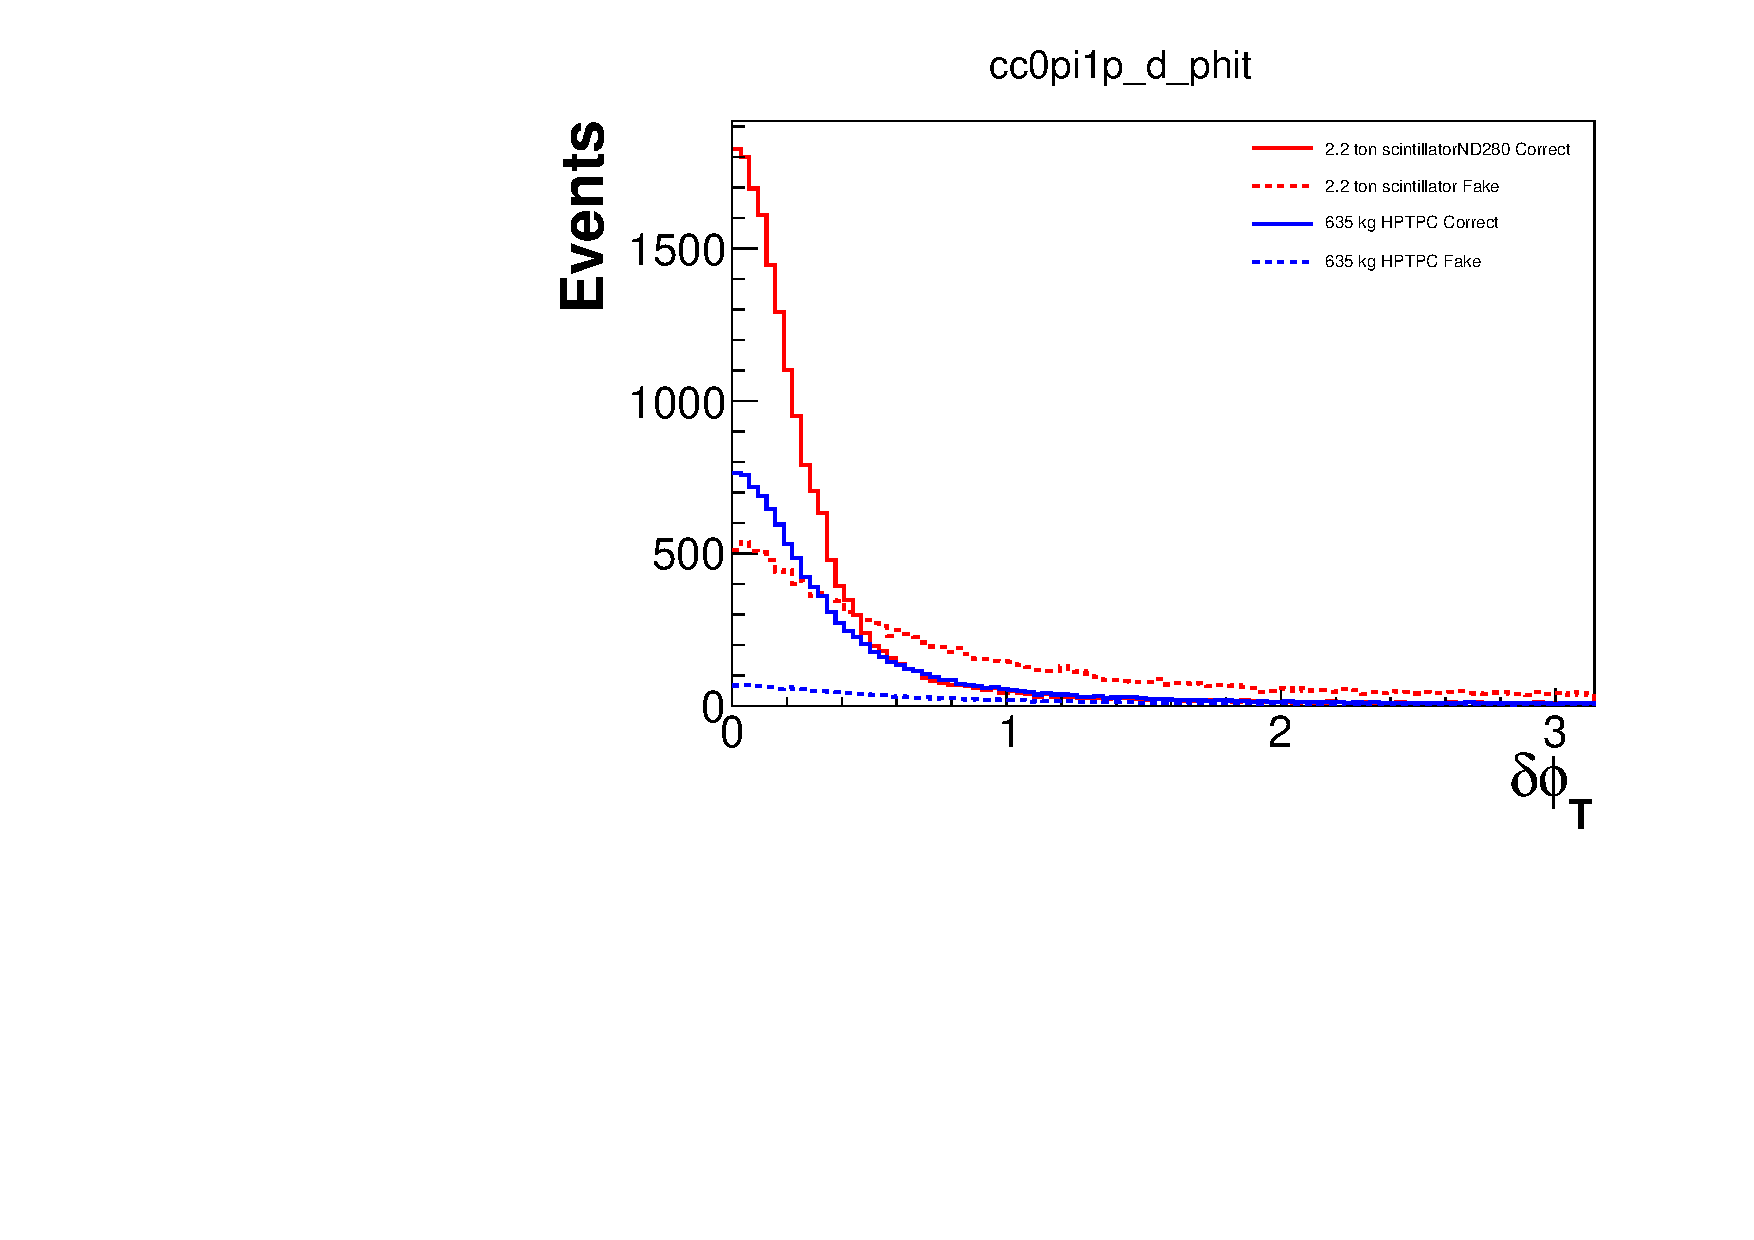
\includegraphics[width=.9\textwidth]{TalkPics/STVforHPTPC_211116/hptpcplots_211116/cc0pi1p_d_phit.pdf}
  \end{frame}

  \begin{frame}
    \frametitle{1D distributions for CC0$\pi$1P}
    \centering
    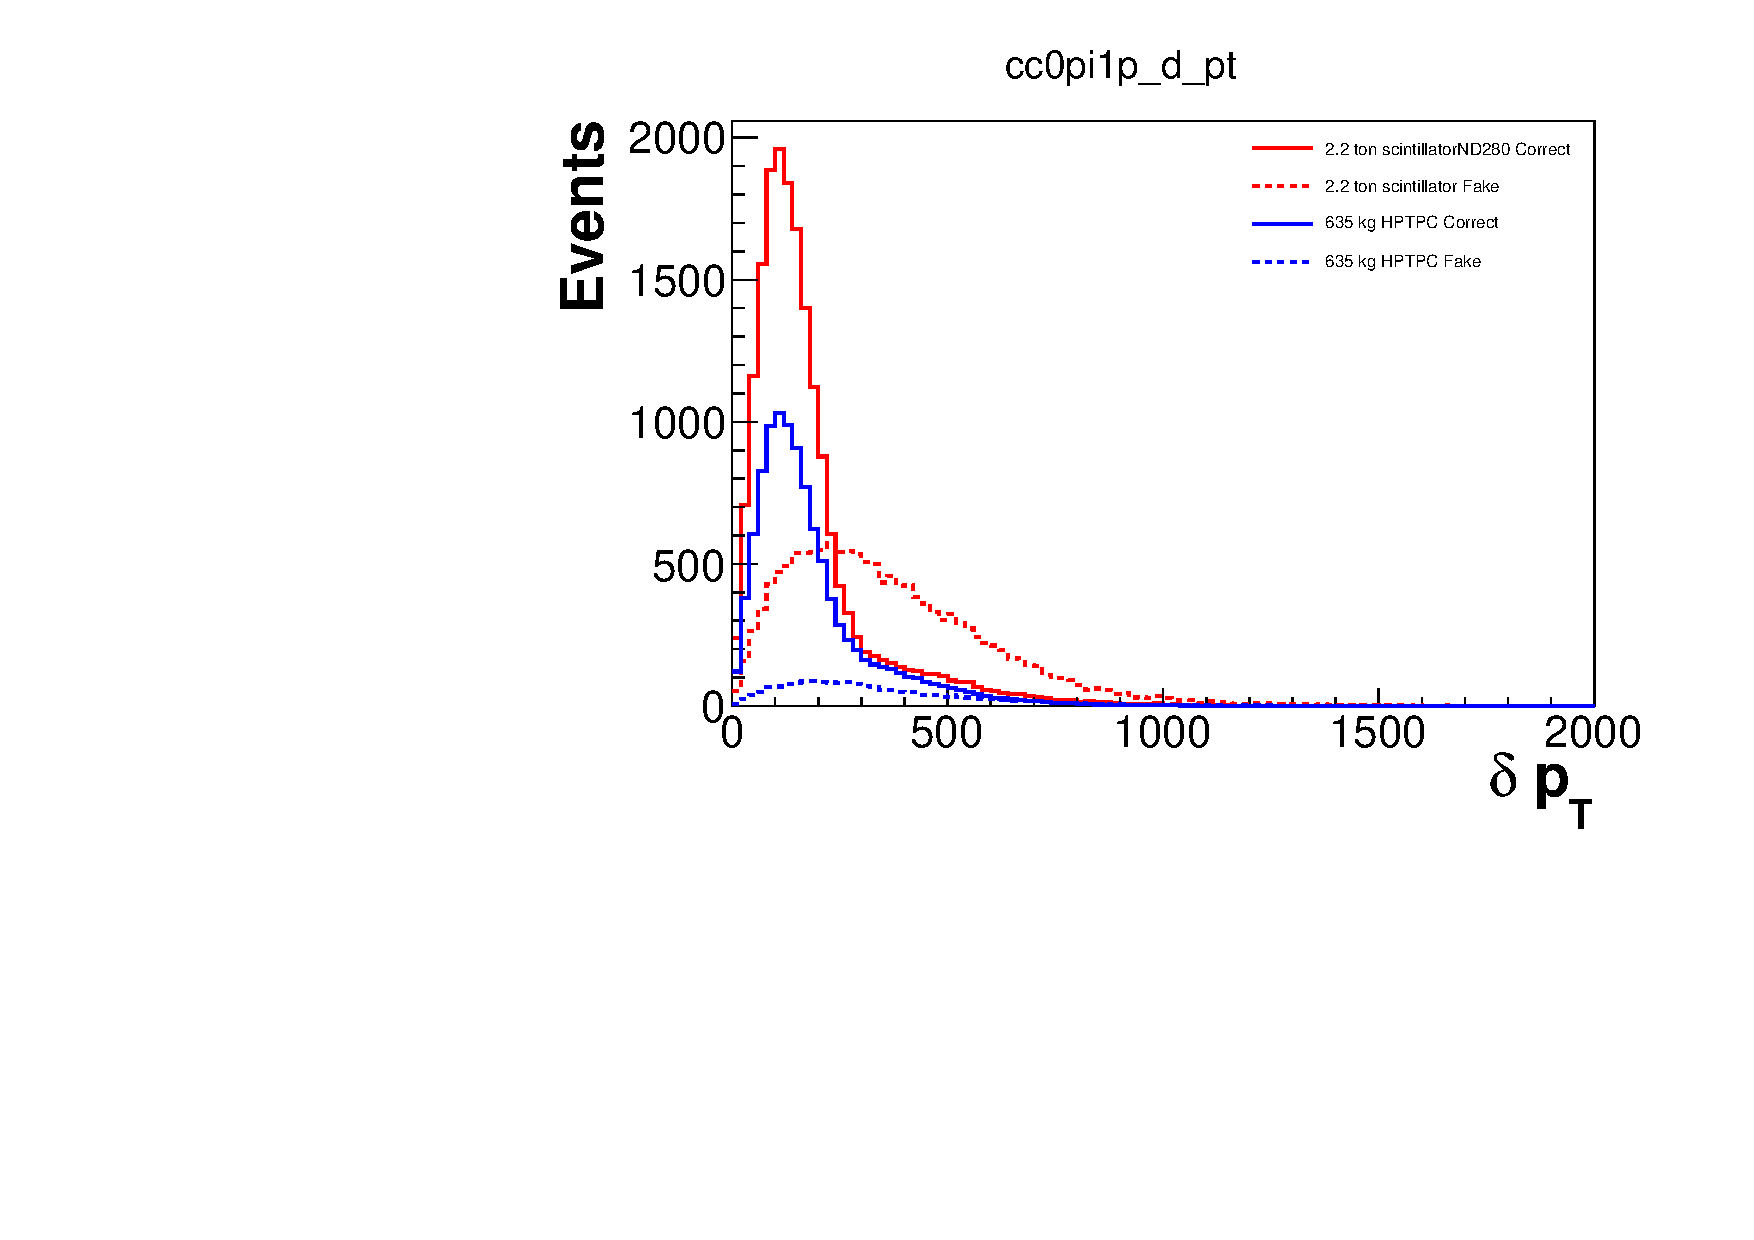
\includegraphics[width=.9\textwidth]{TalkPics/STVforHPTPC_211116/hptpcplots_211116/cc0pi1p_d_pt.pdf}
  \end{frame}

  \begin{frame}
    \frametitle{1D distributions for CC0$\pi$1P}
    \centering
    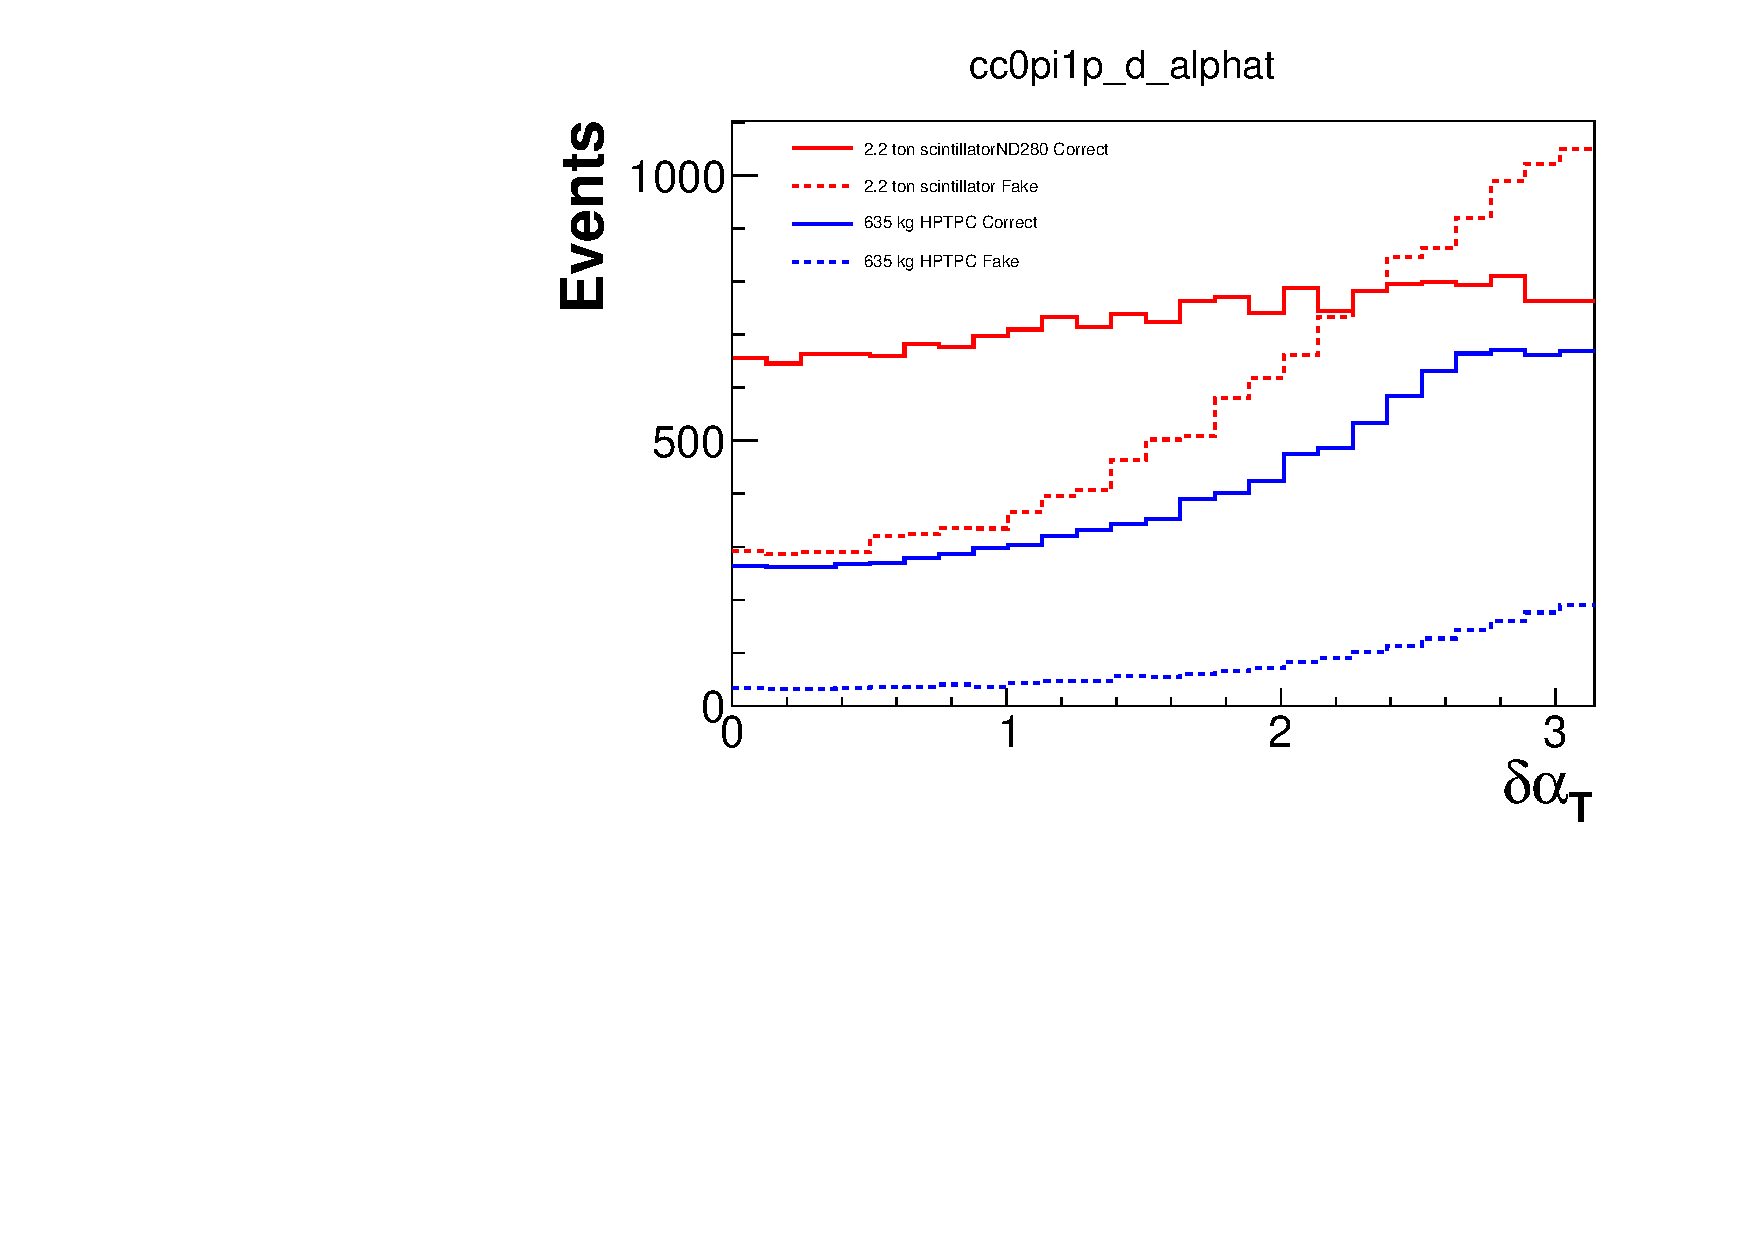
\includegraphics[width=.9\textwidth]{TalkPics/STVforHPTPC_211116/hptpcplots_211116/cc0pi1p_d_alphat.pdf}
  \end{frame}

  \begin{frame}
    \frametitle{2D distribution highlights for CC0$\pi$1P}
    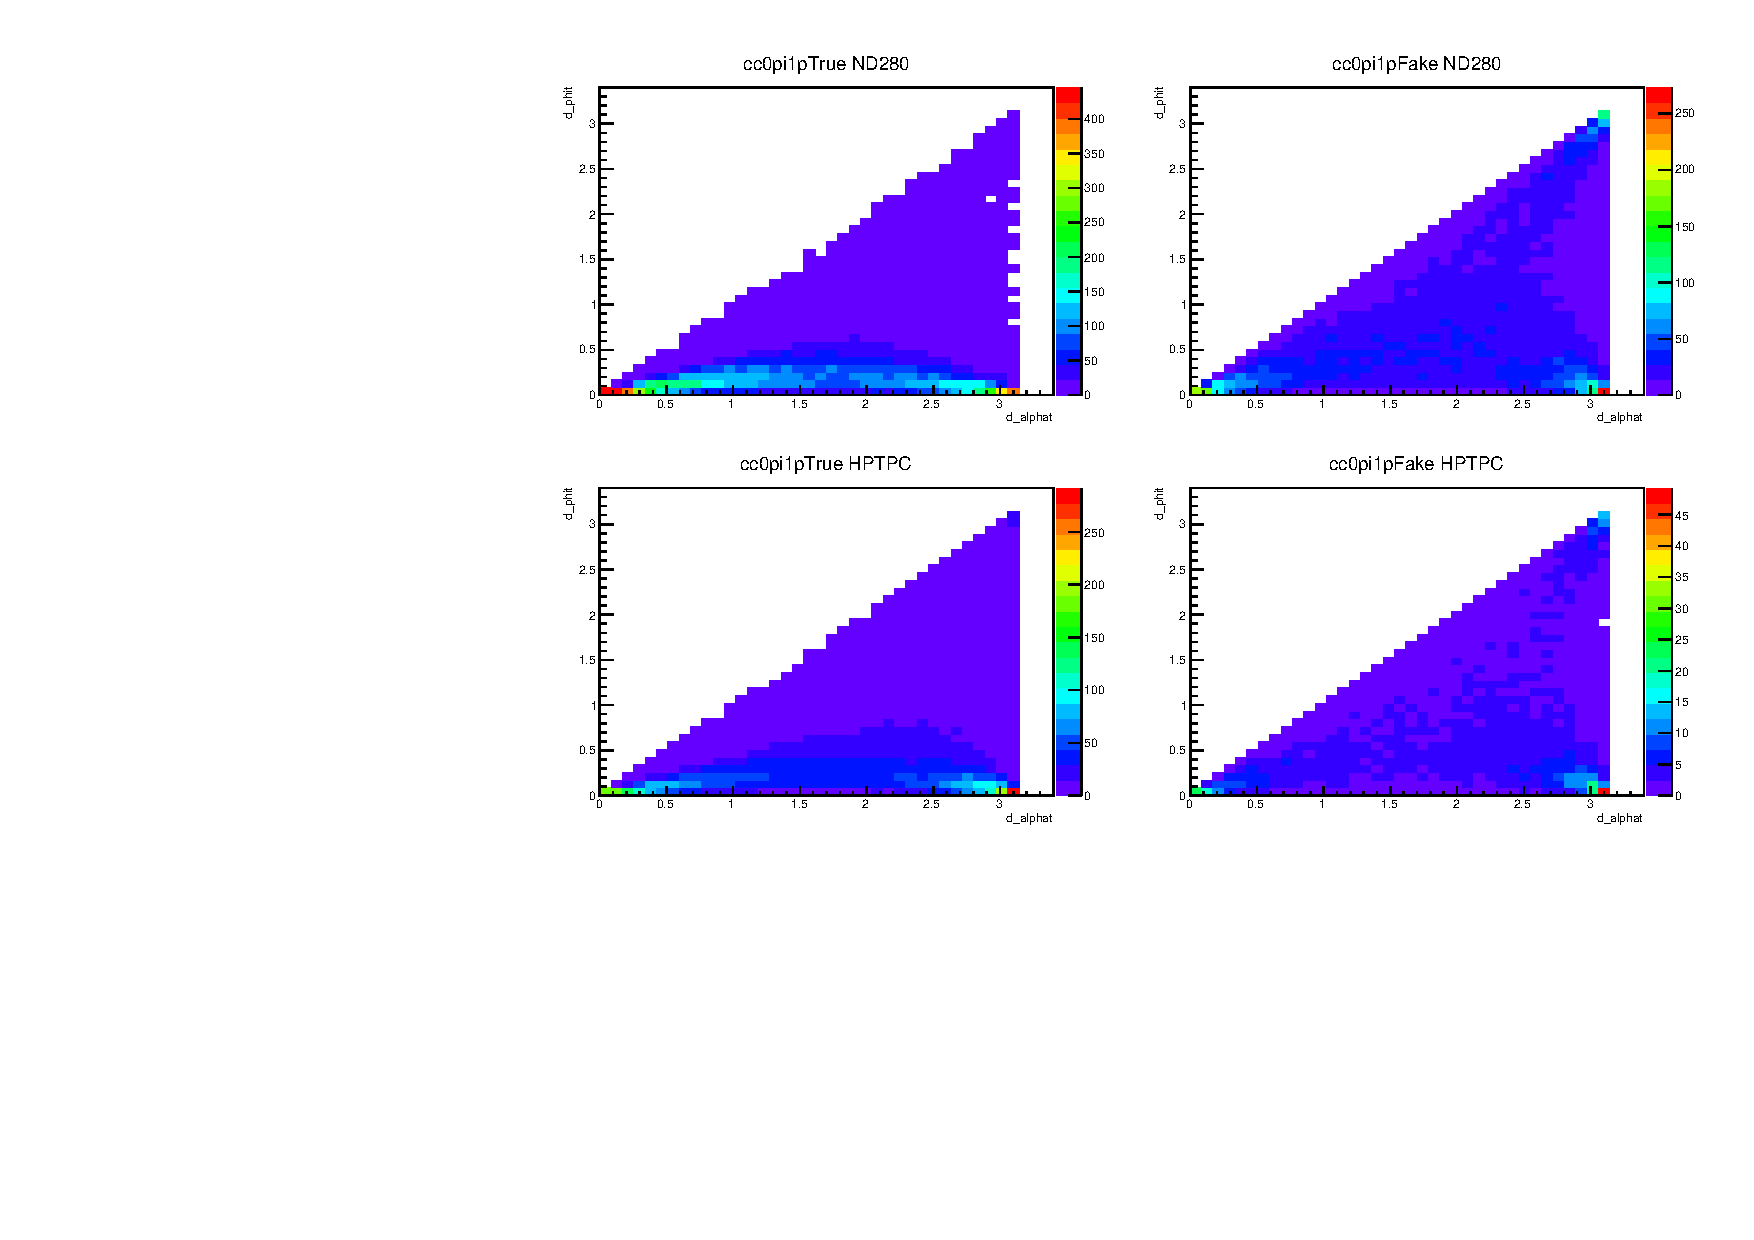
\includegraphics[width=.9\textwidth]{TalkPics/STVforHPTPC_211116/hptpcplots_211116/cc0pi1p_d_phitd_alphat.pdf}
  \end{frame}

  \begin{frame}
    \frametitle{Additional information}
    \begin{itemize}
    \item Particularly for $\delta p_{T}$ context is important
    \end{itemize}
    \begin{block}{}
      \centering
      \begin{fmfgraph*}(60,50)
        \fmftop{i1,m1,m2,m3,m4,m5,m6,m7,o1}
        \fmfbottom{i2,m8,m9,m10,m11,o2}
        \fmf{fermion,tension=4}{v1,i2}
        \fmf{fermion,tension=4}{v1,o2}
        \fmf{fermion}{v1,m1}
        \fmf{dashes}{v1,m3}
        \fmf{fermion}{v1,m4}
        \fmf{fermion}{v1,m5}
        \fmf{fermion}{v1,m6}
        \fmf{fermion}{v1,m7}
        \fmf{fermion}{v1,m8}
        \fmf{fermion}{v1,m9}
        \fmf{fermion}{v1,m10}
        \fmf{fermion}{v1,m11}
      \end{fmfgraph*}
      \hspace{1.5cm}
      VS
      \hspace{1.5cm}
      \begin{fmfgraph*}(60,50)
        \fmftop{i1,m1,m2,m3,m4,m5,m6,m7,o1}
        \fmfbottom{i2,m8,m9,m10,m11,o2}
        \fmf{fermion,tension=4}{v1,i2}
        \fmf{fermion,tension=4}{v1,o2}
        \fmf{fermion}{v1,m1}
        \fmf{dashes}{v1,m3}
      \end{fmfgraph*}
      \vspace{.2cm}
    \end{block}
    \begin{itemize}
    \item Both events have the same $\delta p_{T}$ but this is clearly more significant on the right
    \end{itemize}
    
  \end{frame}

  \begin{frame}
    \frametitle{Additional information}
    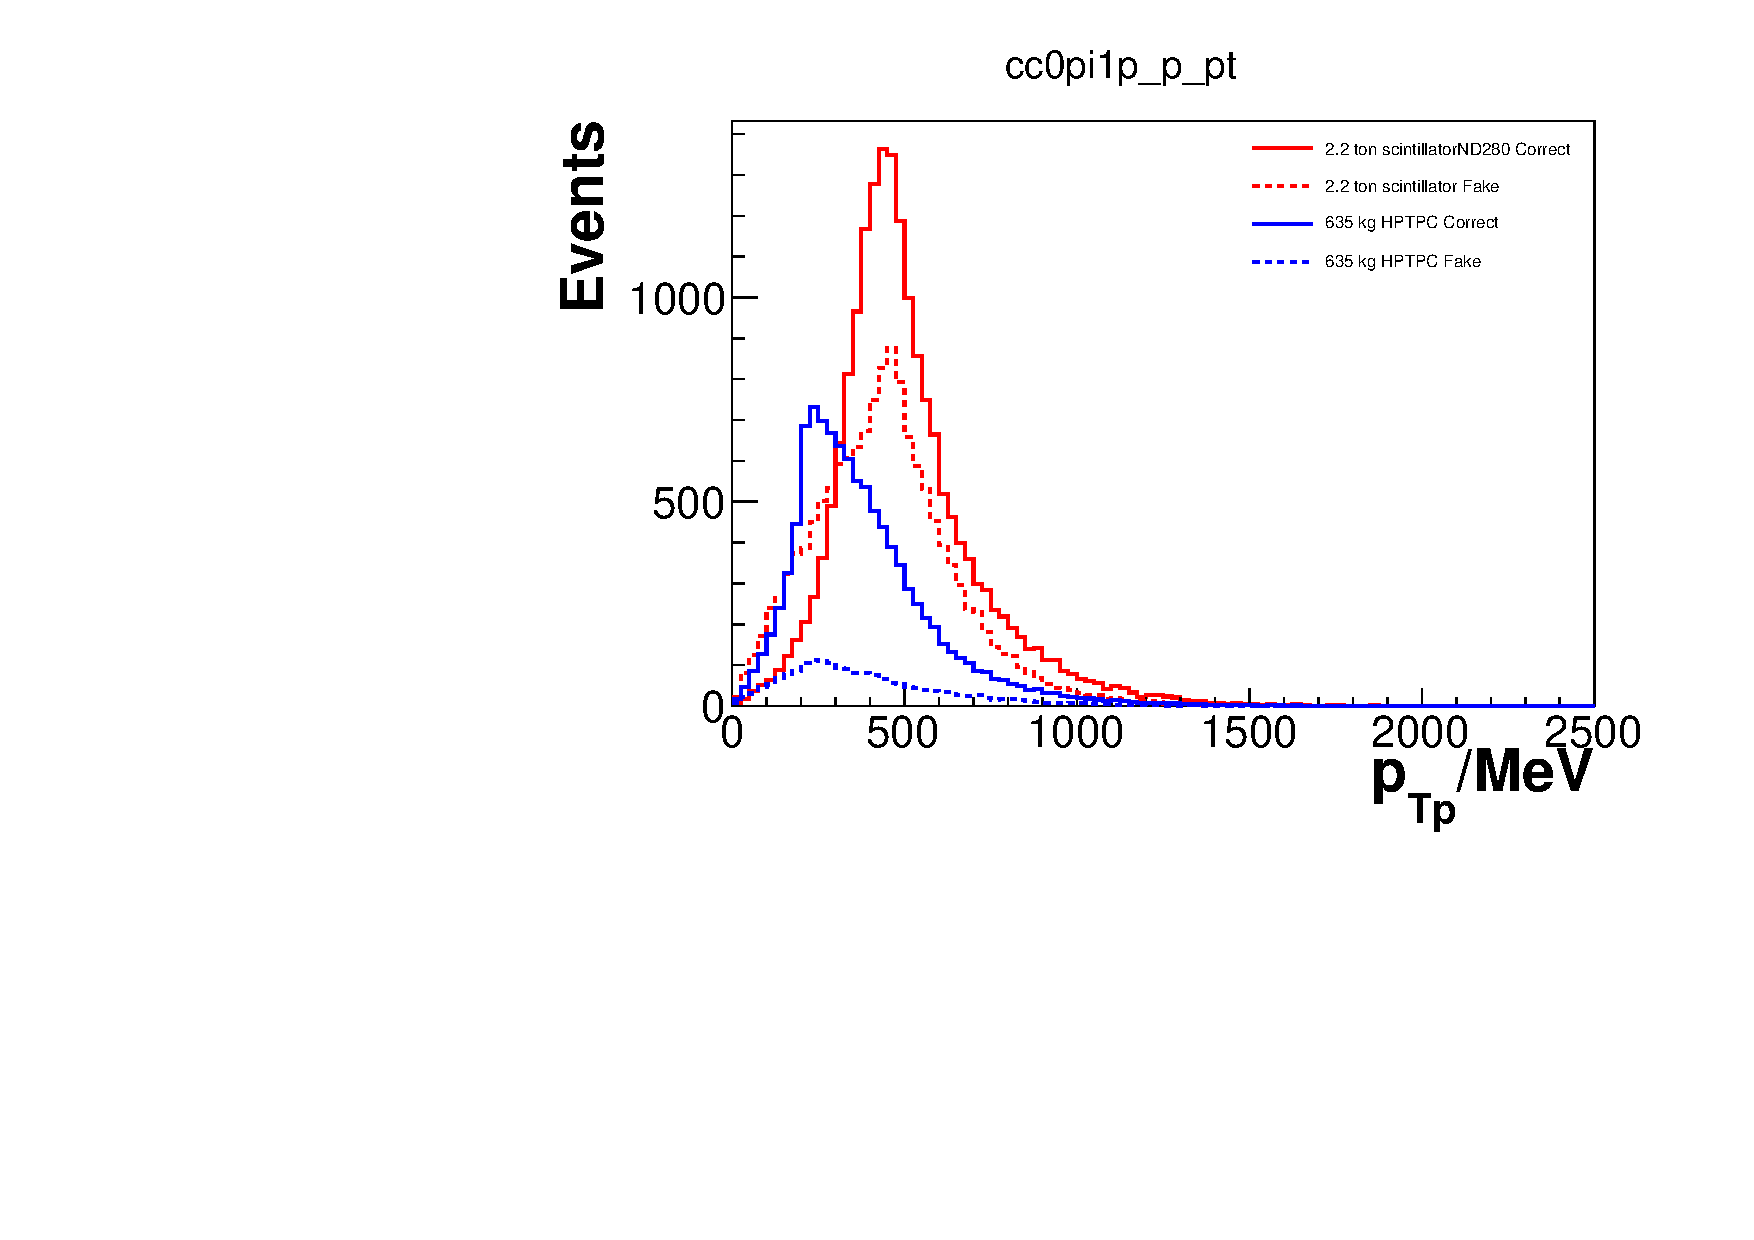
\includegraphics[width=.9\textwidth]{TalkPics/STVforHPTPC_211116/hptpcplots_211116/cc0pi1p_p_pt.pdf}
  \end{frame}

  \begin{frame}
    \frametitle{2D distribution highlights for CC0$\pi$1P}
    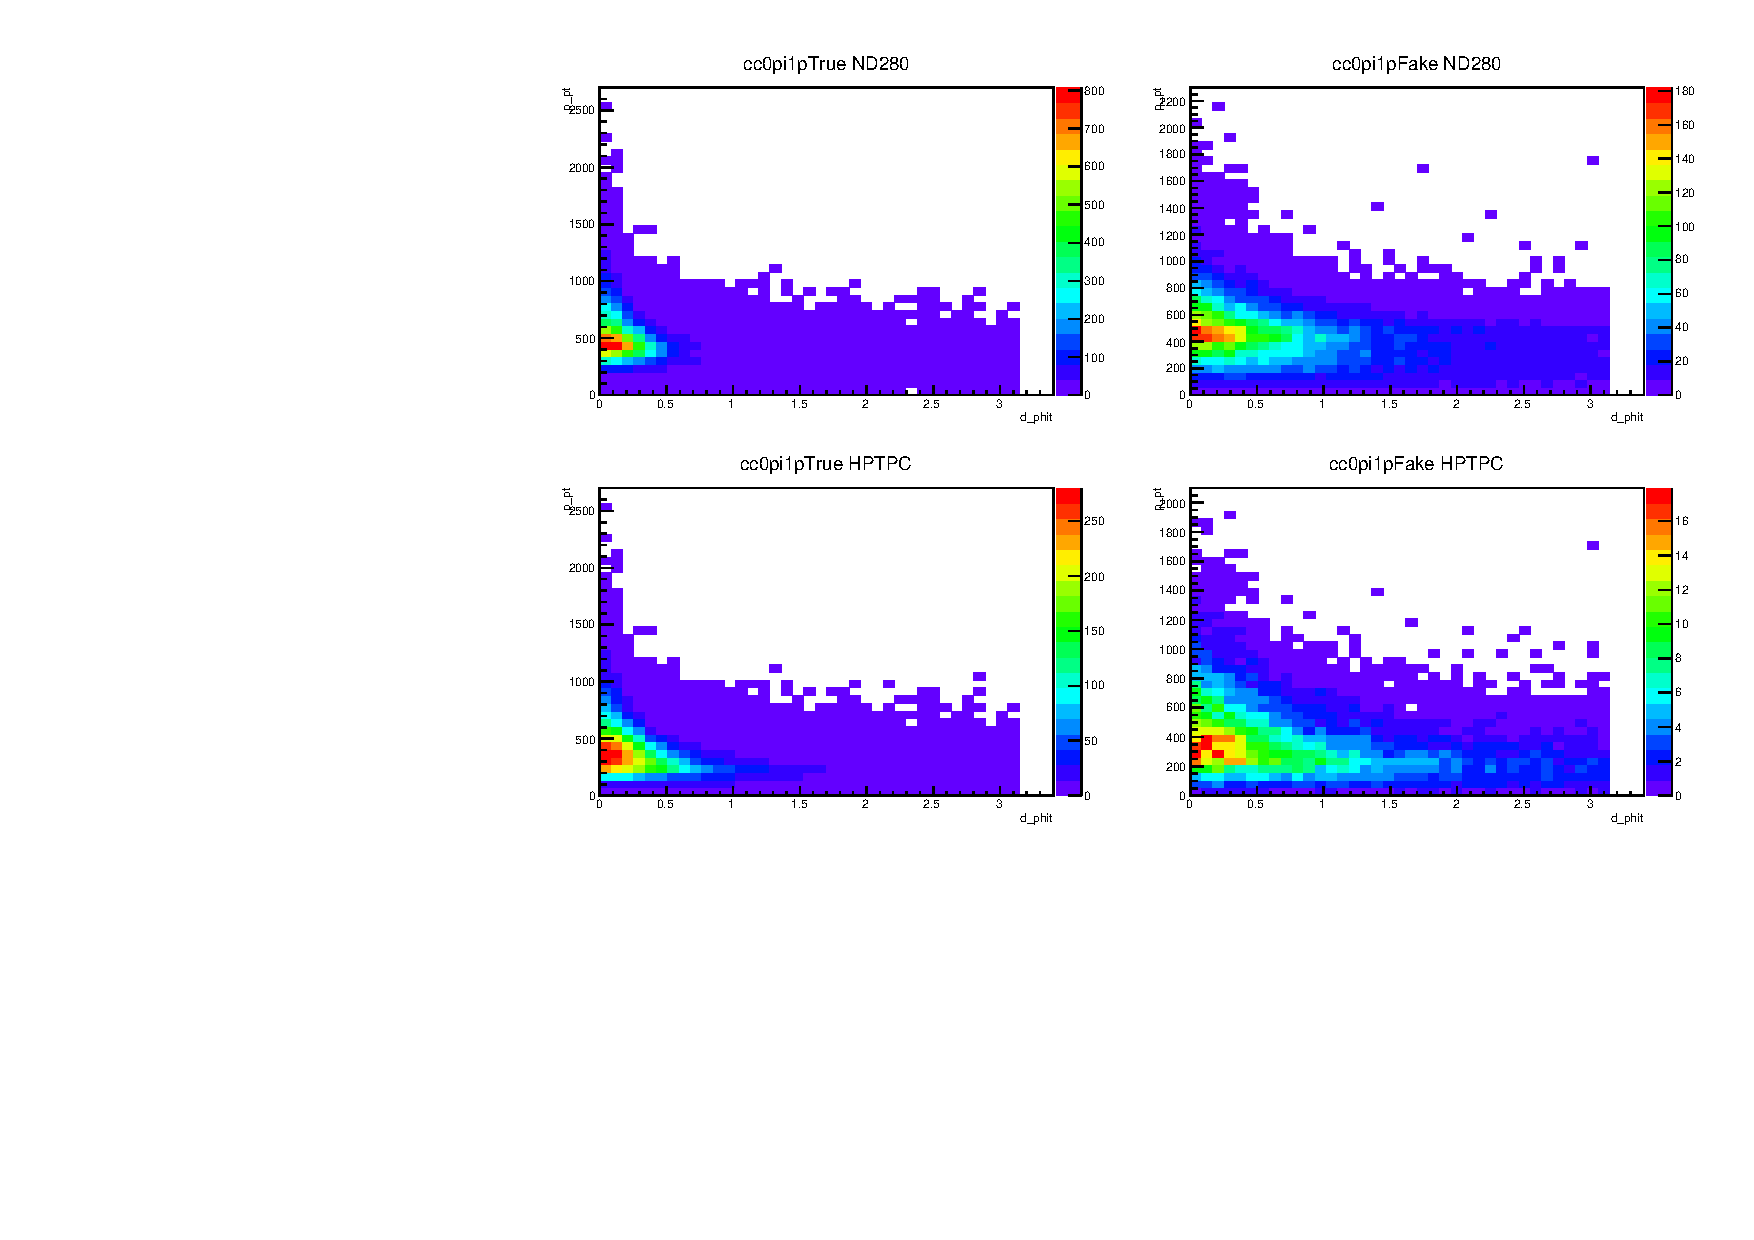
\includegraphics[width=.9\textwidth]{TalkPics/STVforHPTPC_211116/hptpcplots_211116/cc0pi1p_p_ptd_phit.pdf}
  \end{frame}

  \begin{frame}
    \frametitle{2D distribution highlights for CC0$\pi$1P}
    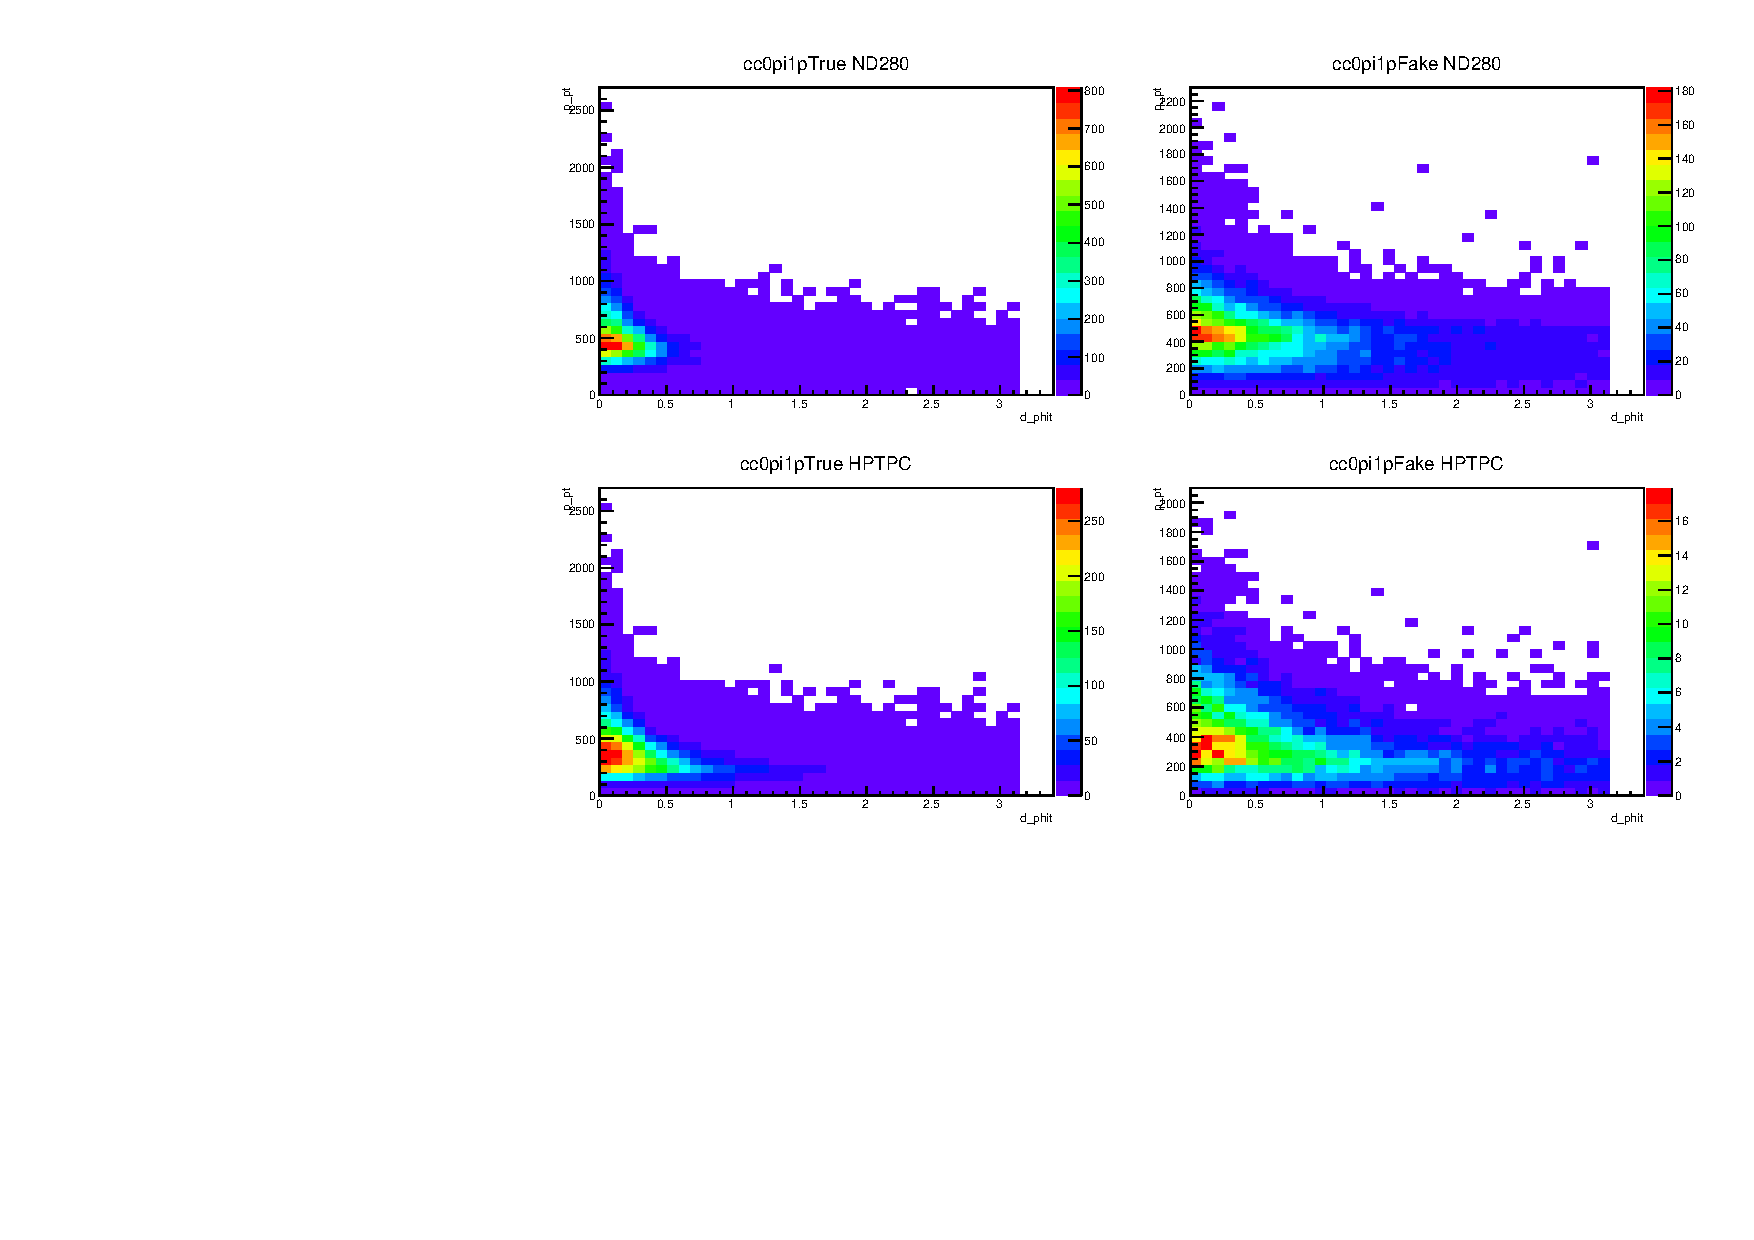
\includegraphics[width=.9\textwidth]{TalkPics/STVforHPTPC_211116/hptpcplots_211116/cc0pi1p_p_ptd_phit.pdf}
  \end{frame}

  \begin{frame}
    \frametitle{}
    \label{lastframe}
    \begin{block}{}
      \begin{itemize}
      \item Transverse variables on their own don't immediately give better signal/background discrimination
      \item Combination with other variables has potential to help with this
      \item Next step is to look at these variables with Mark's fake data studies to determine how transverse variables impact model determination
      \end{itemize}
    \end{block}
  \end{frame}

  %Backup goes here
  
\end{fmffile}
\end{document}

\begin{frame}
\end{frame}
